\section{Elektronik til blyantspidser}
\begin{figure}[h]
	\begin{center}
	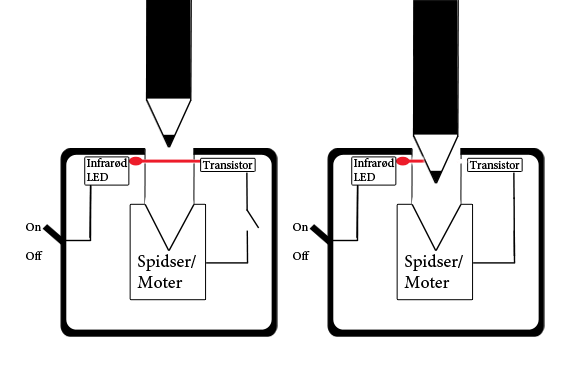
\includegraphics[scale=0.4]{Billeder/illustratzion.png}
	\caption{Illustration af hvorledes blyantspidseren aktiveres}\label{fig:spidser}
	\end{center}
\end{figure}
I nedenstående beskrives hvorledes en elektrisk blyantspidser er blevet automaticeret, så den starter, når en blyant sættes i den. På figur ~\ref{fig:spidser} kan det ses, hvordan det er lavet, så hverken knapper eller andre udefrakommende faktorer skal anvendes for at igangsætte blyantspidseren. Først kommer et afsnit hvor diagrammets opbygning er beskrevet, hvorefter der kommer et afsnit med forklaringer på, hvorfor de forskellige komponenter er anvendt. 

\subsection{Diagram over det elektriske kredsløb}

\begin{figure}[h]
	\begin{center}
	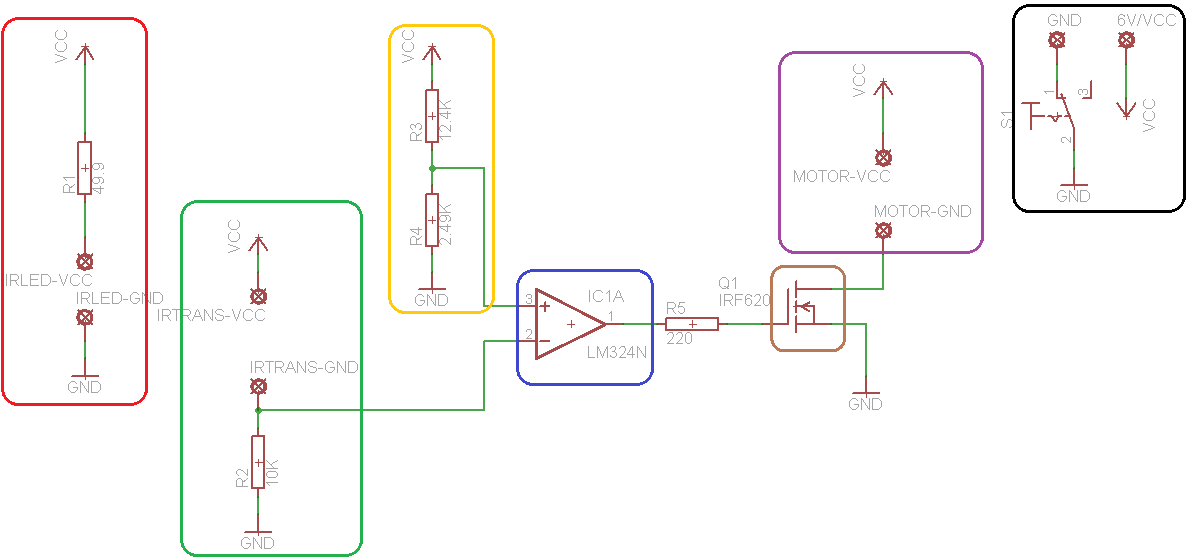
\includegraphics[scale=0.4]{Billeder/Elektronik-schmatic-farver-v2.png}
	\caption{Kredsløbet til blyantspidseren}\label{fig:kredslob}
	\end{center}
\end{figure}

Figur ~\ref{fig:kredslob} illustrerer det elektriske kredsløb i blyantspidseren. LED'en, den lysfølsomme transistor og motoren ses ikke på illustrationen, da disse ikke sidder på printet, men er trukket væk fra printet med ledninger. Det står dog skrevet, hvor i kredsløbet de er placeret. \\
Tilsluttet spændingskilden er en 49.9 \textOmega\
modstand. Denne er serieforbundet med en LED (OP298) der udsender infrarødt lys til en lysfølsom transistor (OP598). Mellem den lysfølsomme transistor og ground, er koblet en 10k \textOmega  modstand. Parallelt med disse er koblet den inverterende terminal af en operationsforstærker (LM324N). På den ikke-inverterende terminal er der tilkoblet to modstande i parallelforbindelse. Disse er dimensioneret til hhv. 12.4k\textOmega\ og 2.49k\textOmega. På outputtet er koblet en 220\textOmega\ modstand, der er forbundet til gate-indgangen på den efterfølgende MOSFET (IRL8113). MOSFET'ens source går til ground, og drain går til blyantspidserens motor som er tilsluttet til vcc som er 6V.\\
Helt ude til højre på figur ~\ref{fig:kredslob} kan man se de to steder hvor ground og 6V er tilsluttet. Mellem ground og vores kredsløb har vi placeret en 3 punkts vippe kontakt. \\


 